% !TeX root = vpl.tex

\chap{States (Advanced Mode)}\label{ch.states}

A program in VPL is a list of event-actions pairs. \emph{All} the events
are checked periodically and the appropriate actions are taken. This
limits the programs that we can create. To develop more complex
programs, we need a way to specify that some event-actions pairs are
active, while others are not.

For example, in the line-following program in \cref{ch.line}, when the
robot runs off the tape, we want it to turn left or right to search for
the tape with the direction depending on which side it ran off. There
will be two event-actions pairs: one to turn left when the robot runs
off the right of the tape and one to turn right when it runs off the
left of the tape.

%\informationbox{Advanced mode}{States are supported in \emph{advanced
%mode}. Click on \blkmed{advanced} to enter advanced mode.}

\sect{Tap, tap}

In many programs, we used one button to start the robot's behavior and
another to stop it. Consider, though, the power switch on a computer.
The same switch is used to turn the computer on and off; the computer
\emph{remembers} whether it is in the state \bu{on} or the state
\bu{off}.

Write a program that turns the robot's lights on when it is tapped and
turns them off when tapped again.

{\raggedleft \hfill Program file \bu{tap-on-off.aesl}}

It is convenient to display the required behavior in a \textit{state diagram}:

\begin{center}
\begin{picture}(240,45)
\thicklines
%\put(0,0){\framebox(240,40){}}
\put(20,20){\circle{40}}
\put(0,0){\makebox(40,40){\textsf{off}}}
\put(220,20){\circle{40}}
\put(200,0){\makebox(40,40){\textsf{on}}}
\put(40,30){\vector(1,0){160}}
\put(0,30){\makebox(240,10){\textsf{tap $\rightarrow$ turn on}}}
\put(200,10){\vector(-1,0){160}}
\put(0,10){\makebox(240,10){\textsf{tap $\rightarrow$ turn off}}}
\end{picture}
\end{center}

In the diagram there are two states indicated by circles labeled with
the names of the states \bu{off} and \bu{on}. From state \bu{off} the
robot can go to state \bu{on} and back, but only by following the
instructions on the arrows. The instructions describe when a transition
from one state to another can occur and what happens when it does occur:

\begin{itemize}

\item \emph{When} the robot is in state \bu{off} \textbf{\textit{and}}
the \emph{tap} event occurs $\rightarrow$ turn the lights \emph{on}
\textbf{\textit{and}} go to state \bu{on}.

\item \emph{When} the robot is in state \bu{on} \textbf{\textit{and}}                                                                                                                        
the \emph{tap} event occurs $\rightarrow$ turn the lights \emph{off}                                                                                                                         
\textbf{\textit{and}} go to state \bu{off}. 

\end{itemize}

The emphasized word \textbf{\textit{and}} before the arrow~$\rightarrow$
means that there are \emph{two conditions} that must be true in order
for the transition to be taken. (a) The robot must be in a certain state
and (b) the event must occur. When both conditions are true, the
transition is taken, causing both the state to change and the action
written after the arrow~$\rightarrow$ to be performed.

It is important to realize that the two parts of the condition are
independent. In the above diagram (repeated here), the event \emph{tap}
appears twice, but the action caused by the occurrence of this event
\emph{depends on which state the robot is in}.

\vspace*{-1ex}

\begin{center}
\begin{picture}(240,40)
\thicklines
%\put(0,0){\framebox(240,40){}}
\put(20,20){\circle{40}}
\put(0,0){\makebox(40,40){\textsf{off}}}
\put(220,20){\circle{40}}
\put(200,0){\makebox(40,40){\textsf{on}}}
\put(40,30){\vector(1,0){160}}
\put(0,30){\makebox(240,10){\textsf{tap $\rightarrow$ turn on}}}
\put(200,10){\vector(-1,0){160}}
\put(0,10){\makebox(240,10){\textsf{tap $\rightarrow$ turn off}}}
\end{picture}
\end{center}

\vspace*{-1ex}

In a single state, different events can cause different actions and
different transitions. In the following diagram, touching the left
button in the state \textbf{off} causes the green light to be turned on
and a change to state \textbf{on1}, while touching the right button
\emph{in the same state} causes a different action, the red light is
turned on, and a change to a different state, \textbf{on2}.

\vspace*{-1ex}

\begin{center}
\begin{picture}(240,80)
\thicklines
%\put(0,0){\framebox(240,80){}}
\put(30,42){\circle{30}}
\put(14,28){\makebox(30,30){\textsf{off}}}
\put(220,22){\circle{30}}
\put(205,8){\makebox(30,30){\textsf{on2}}}
\put(40,57){\vector(1,0){160}}
\put(220,60){\circle{30}}
\put(205,45){\makebox(30,30){\textsf{on1}}}
\put(40,27){\vector(1,0){160}}
\put(0,60){\makebox(240,10){\textsf{left button $\rightarrow$ turn green}}}
\put(0,30){\makebox(240,10){\textsf{right button $\rightarrow$ turn red}}}
\end{picture}
\end{center}

\vspace*{-4ex}

\sect{Implementing state diagrams with event-actions pairs}

\Cref{fig.turn-on-off} shows the implementation of the behavior
described in the state machine above. The left circle in the block \blksm{event-tap} is
checked (and is displayed in red) to indicate that this is a block for
the tap event.

\importantbox[The tap block in advanced mode]{The block for the tap event is
different in advanced mode, because it is also used for accelerometer
events as described in \cref{ch.angles}.}

%\begin{figure}
%	\subfigure[Tap to turn on and off]{
%		\label{fig.turn-on-off1}
%		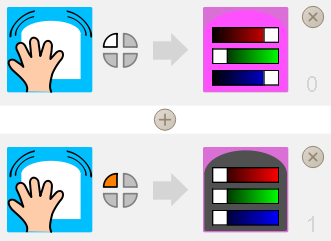
\includegraphics[width=.4\textwidth]{tap-on-off1}
%	}
%	\hfill
%	\subfigure[Tap to change the state]{
%		\label{fig.turn-on-off2}
%		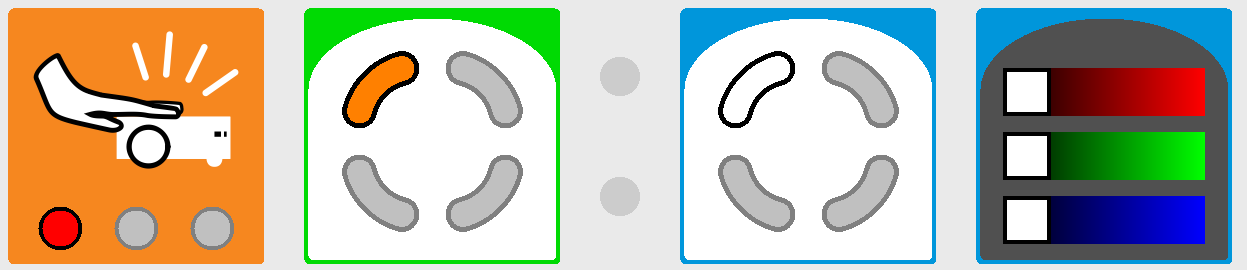
\includegraphics[width=.4\textwidth]{tap-on-off2}
%	}
%	\caption{Tap has a different result depending on a state}
%	\label{fig.turn-on-off}
%\end{figure}
%
%\begin{figure}
%	\subfigure[Tap to turn on and off]{
%		\label{fig.turn-on-off1}
%		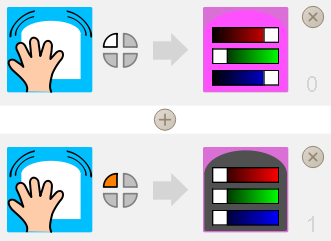
\includegraphics[width=.4\textwidth]{tap-on-off1}
%	}
%	\hfill
%	\subfigure[Tap to change the state]{
%		\label{fig.turn-on-off2}
%		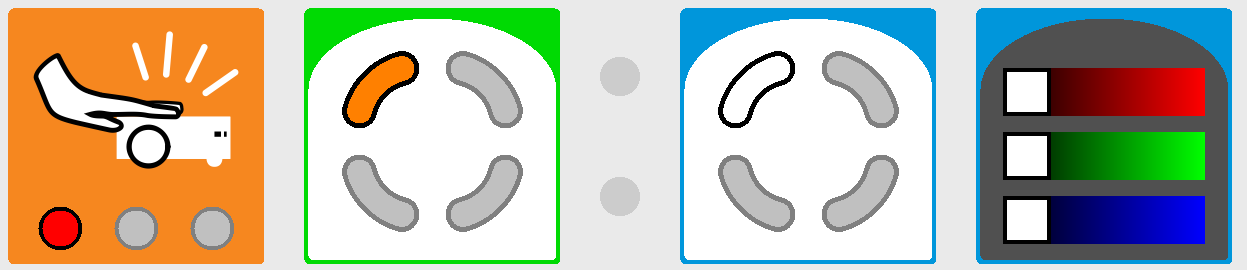
\includegraphics[width=.4\textwidth]{tap-on-off2}
%	}
%	\caption{Tap has a different result depending on a state}
%	\label{fig.turn-on-off}
%\end{figure}

\begin{figure}
\subfigure[Tap to turn the light one]{
\label{fig.turn-on-off1}
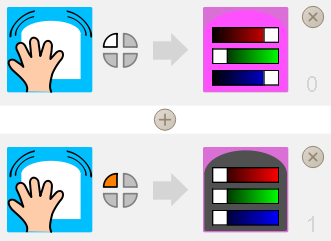
\includegraphics[width=.6\textwidth]{tap-on-off1}
}
\subfigure[Tap to turn the light off]{
\label{fig.turn-on-off2}
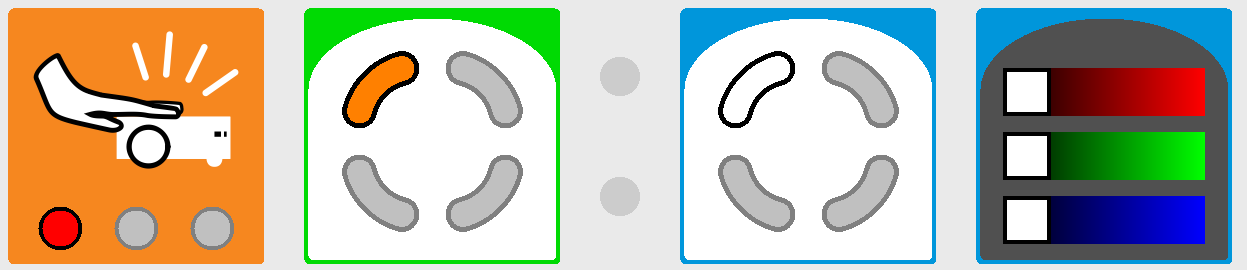
\includegraphics[width=.6\textwidth]{tap-on-off2}
}
\caption{Tap has a different result depending on the state}
\label{fig.turn-on-off}
\end{figure}

In the first event-actions pair (\cref{fig.turn-on-off1}), the event is
composed of the tap block together with an indication of the state
\blksm{state-filter}. A state is indicated by four quarters of a circle,
each of which can be either on (orange) or off (white). In this program,
we will use the upper-left quarter to indicate whether the robot's top
light is off or on. In \cref{fig.turn-on-off1}, this quarter is colored
white, meaning that the robot's light is off. Therefore, the meaning of
the this pair is: \textbf{if} the robot is tapped \textbf{and} the light
is off, \textbf{then} turn the light on.

For the second event-actions pair (\cref{fig.turn-on-off2}), the quarter
is colored orange, indicating that the robot's light is on. The meaning
of pair is: \textbf{if} the robot is tapped \textbf{and} the light is
on, \textbf{then} turn it off.

If you look again at the state diagram, you will see that only half the
job is done. When turning the light on or off, we also have to change
the state of the robot from \bu{off} to \bu{on} or from \bu{on} to
\bu{off}. Therefore, we need to add a \emph{state} action block
\blksm{action-states} to each pair. This block changes the state as
indicated by the quarters that are white or orange.

We can summarize the meaning of the program in \cref{fig.turn-on-off}
as follows:

\begin{quote}
\emph{When} the robot is tapped \emph{and} the state is \bu{off},\\
change the state to \bu{on} \emph{and} turn the top light \bu{on}.

\emph{When} the robot is tapped \emph{and} the state is \bu{on},\\
change the state to \bu{off} \emph{and} turn the top light \bu{off}.
\end{quote}

Each event causes both an action on the light and a change of the state
of the robot. The actions depend on the \emph{current} state of the robot.

\sect{How many states can the robot be in?}

When used in an event state block or in the action state block, each quarter can be:
\begin{itemize}
\item \textbf{White}: the quarter is \emph{off};
\item \textbf{Orange}: the quarter is \emph{on};
\item \textbf{Gray}: the quarter is ignored.
\end{itemize}

For example, in \blksm{states}, the upper-left and lower-right quarters
are on, the upper-right one is off and the lower-left one is not taken
into account, meaning that if \blksmpure{states} is associated with an
event block, the event will occur if the state is either set to:
\begin{center}
\centering
\makebox{\raisebox{-1.7em}{
\includegraphics[height=4em]{states1}}}\quad or \quad%
\makebox{\raisebox{-1.7em}{
\includegraphics[height=4em]{states2}}}
\end{center}

Since each of the four quarters can be either on or off, there are 2
$\times$ 2 $\times$ 2 $\times$ 2 = 16 states:
\begin{quote}
\bu{(off, off, off, off), (off, off, off, on), (off, off, on, off),\\
\mbox{}\hspace{3em}\ldots\\
(on, on, off, on), (on, on, on, off), (on, on, on, on)}.
\end{quote}
\Cref{fig.all-states} displays these 16 possible states.

\importantbox{The current state of the robot is displayed in the four
diagonal segments of the light circle on the top of the robot.
\cref{fig.state-leds} shows the robot in the state \bu{(on, on, on,
on)}.}

\trickbox[Information]{When a program is run, the initial state is
\bu{(off, off, off, off)}:\quad \blkmed{state-all-off}}

\trickbox{If you do not use all possible 16 states, but only 2 or 4, for
example, you are free to decide which quarters you use to represent your
state. In addition, if you have two different things you want to encode,
and each of them has two possible values, you can use two quarters
independently. That is why the ability to \emph{ignore} a quarter is
very useful! }

\begin{figure}
\subfigure[All possible states of Thymio]{
\label{fig.all-states}
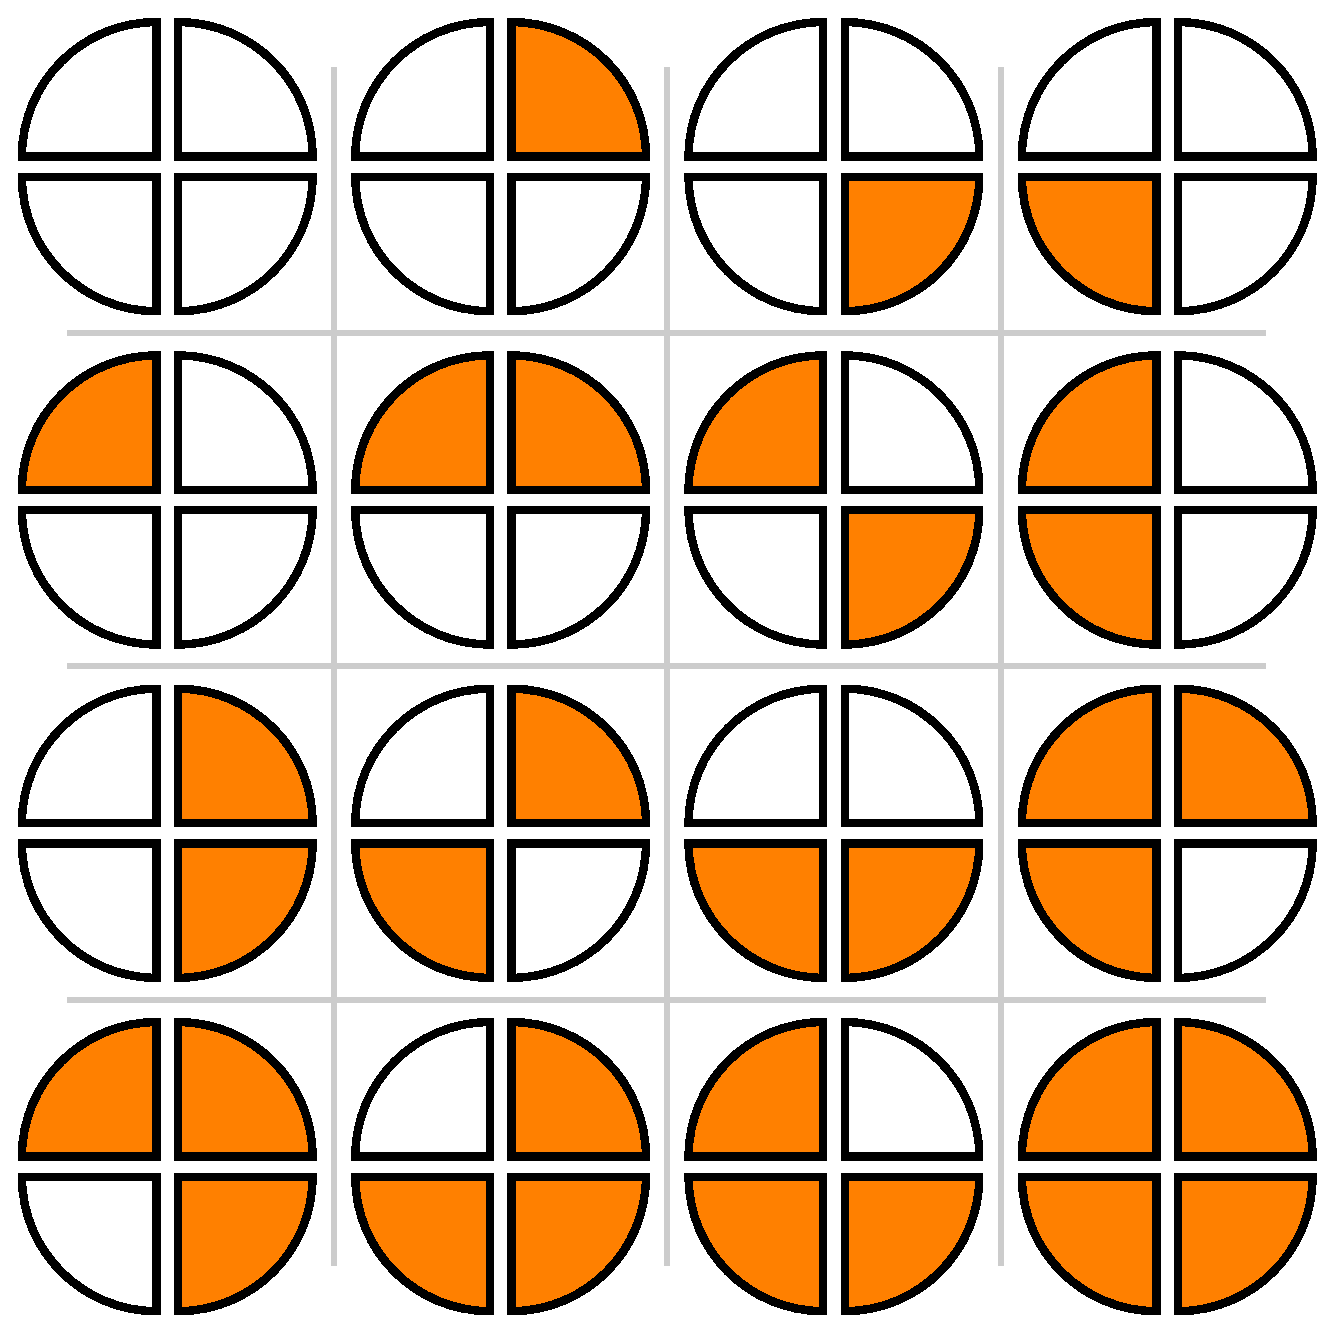
\includegraphics[width=.4\textwidth]{all-states}
}
\hfill
\subfigure[The light circle indicates the state]{
\label{fig.state-leds}
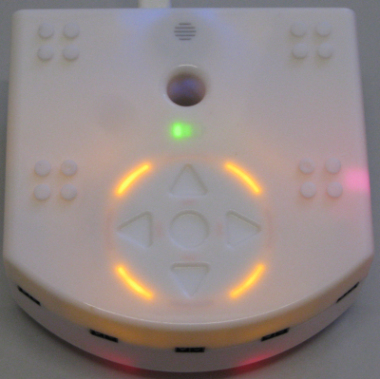
\includegraphics[width=.4\textwidth]{state-leds}
}
\caption{The states of Thymio and their representation}
\end{figure}

\sect{Get the mouse}

Write a program to implement the behavior of a cat searching for a mouse:
When the center button is touched, the robot turns counterclockwise
(from right to left), searching for a mouse. If the robot detects a
mouse with its rightmost sensor, it turns clockwise (from left to right)
until the mouse is detected by its center sensor, at which point it
stops (\cref{fig.cat-mouse}).

{\raggedleft \hfill Program file \bu{mouse.aesl}}

The following state diagram describes the behavior of the robot:

\begin{center}
\unitlength=1.2pt
\begin{picture}(320,35)
%\put(0,0){\framebox(320,35){}}
\put(40,10){\oval(80,20)}
\put(160,10){\oval(80,20)}
\put(280,10){\oval(80,20)}
\put(0,0){\makebox(80,20){\bu{search left}}}
\put(120,0){\makebox(80,20){\bu{search right}}}
\put(240,0){\makebox(80,20){\bu{found}}}
\put( 80,10){\vector(1,0){40}}
\put(200,10){\vector(1,0){40}}
\put(40,35){\vector(0,-1){15}}
\end{picture}
\end{center}

\begin{enumerate}
\item When the center button is touched, the robot enters the state
\bu{search left} and moves from right to left.
\item When the robot is in state \bu{search left}
and it detects the mouse in the rightmost sensor,
it changes to state \bu{search right} and moves from left to right.
\item When the robot is in state \bu{search right}
and it detects the mouse in the center sensor,
it changes to state \bu{found} and stops.
\end{enumerate}

The important point to notice is that when the mouse is detected by the
center sensor, it stops \emph{only if} the robot is in state \bu{search
right}. Otherwise (if the mouse is detected by the center sensor when
the robot is in state \bu{search left}), nothing happens.

%\begin{figure}
%\subfigure[The cat has found the mouse]{\label{fig.cat-mouse}
%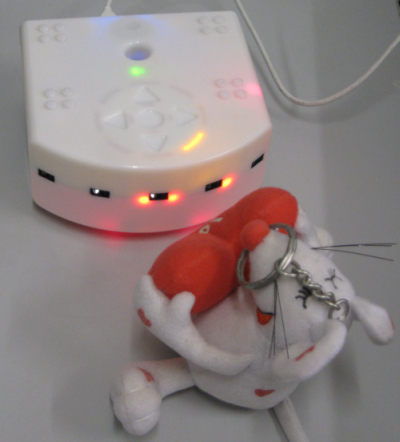
\includegraphics[width=0.4\textwidth]{cat-mouse}}
%%	\hfill
%\subfigure[Searching with the rightmost sensor]{\label{fig.mouse2}
%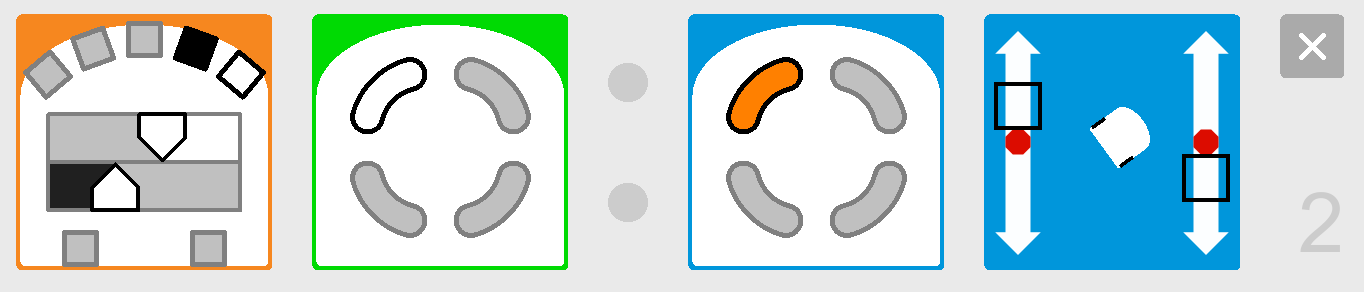
\includegraphics[width=0.6\textwidth]{mouse2}}
%\caption{The robot cat is looking for the mouse}
%\end{figure}

\begin{figure}
\begin{center}
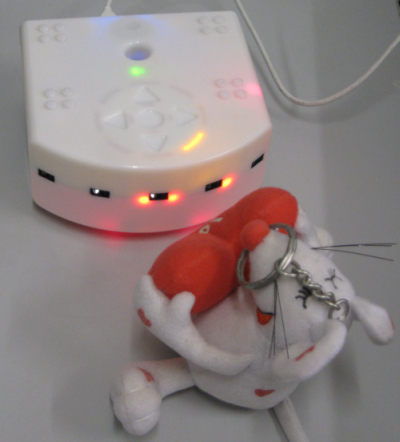
\includegraphics[width=0.4\textwidth]{cat-mouse}
\caption{The robot cat is looking for the mouse}\label{fig.cat-mouse}
\end{center}
\end{figure}

Let us now implement this behavior. We represent the state of the robot
by the upper-left quarter of the state indicator. We choose white for
the state \bu{search left} and orange for the state \bu{search right}.
Since the program ends when the mouse is detected in state \bu{search
right}, we don't need to represent state \bu{found} explicitly.
Initially, all the quarters are \bu{off} (white).

The following event-actions pair implements the behavior in step 1:
\blkc{mouse1}
When the center button is touched, the state changes to \bu{search left}
\emph{and} the robot turns to the left.

The event-actions pair that implements step 2 is:
\blkc{mouse2}
When the mouse is detected by the rightmost sensor while in state
\bu{search left}, the state changes to \bu{search right} \emph{and} the
robot turns to the right.

The small square next to the rightmost sensor is set to black so that
the event occurs only when the rightmost sensor alone detects the mouse.

Step 3 is implemented by the following event-actions pair:
\blkc{mouse3}
When the mouse is detected by the center sensor while 
in state \bu{search right}, the robot stops. 


\trickbox{
You will have to experiment with the distance of the mouse to the robot.
If it is too close to the robot, the sensors on either side of
the central sensor will also detect the mouse, while the event requires
that they \emph{not} detect it.}

\bigskip

\bigskip

\exercisebox{\thechapter.1}{
Write a program that causes the robot to dance: it turns left in
place for two seconds and then turns right in place for three seconds.
These movements are repeated indefinitely.
}

\bigskip

\exercisebox{\thechapter.2 (Difficult)}{
Modify the line-following program from \cref{ch.line} so that the
robot turns left when it leaves the right-hand side of the line and
turns right when it leaves the left-hand side of the line.
}
